
\documentclass[11pt, a4paper]{article}
%\usepackage{proj1}
\usepackage{natbib}
\usepackage{fancyhdr}  
\usepackage{subcaption}
\usepackage{caption}
\usepackage{graphicx}
\linespread{1.25} 
\setlength{\parindent}{0cm}
\graphicspath{{Images/}}
\usepackage{hyperref}
\usepackage{amsmath}
\usepackage{amsfonts}
\usepackage{amssymb}
\usepackage{amsthm}
\usepackage{mathtools}
\usepackage{commath}
\usepackage[warning,debug,nosepfour,autolanguage]{numprint}

%\usepackage[sc,osf]{mathpazo}
\usepackage{subcaption}
\usepackage[a4paper, top=1in, left=1.0in, right=1.0in, bottom=1in, includehead, includefoot]{geometry} %Usually have top as 1in

\usepackage{listings}
\usepackage{color} %red, green, blue, yellow, cyan, magenta, black, white
\definecolor{mygreen}{RGB}{28,172,0} % color values Red, Green, Blue
\definecolor{mylilas}{RGB}{170,55,241}


\hypersetup{colorlinks,linkcolor={black},citecolor={blue},urlcolor={black}}
\usepackage{color}
\urlstyle{same}


\theoremstyle{definition}
\newtheorem{definition}{Definition}[section]

\title{Exact Solutions for the Full Problem \\with Force Control and with Flow Control}
\date{}
%\newcommand{\Sta}{\rho}
\newcommand{\Adj}{p}
\newcommand{\adj}{q}
%\newcommand{\Con}{u}
\newcommand{\Sta}{\rho}
\newcommand{\Stav}{\mathbf{v}}
\newcommand{\Adja}{\mathbf{p}_\Sigma}
\newcommand{\Adjb}{q}
\newcommand{\Adjc}{p_{\partial \Sigma}}
\newcommand{\Con}{\mathbf{f}}
\newcommand{\nor}{\mathbf{n}}

\pagenumbering{gobble}
\begin{document}
	- Dante: where does the 1/2 come from??\\
	\\
	- BCs?\\
	- Dt?\\
	-$\nabla \Stav$ transpose implementation\\
	- division by rho?\\
	- 'good' test problem?\\
    - what is a small beta here?\\
    - naming convention for things?\\
    - I think that maybe high friction is good for the FW problem but bad for the adjoint. Not 100 percent sure but it looks a bit like this...\\
    - Convergence fluctuates (FixPt) -- never did this in the AD problems. Why?\\
    - Fun 1 worked with friction = 5 and beta = 10 but not for lower beta\\
    - I think solving 4 instead of 2 PDEs makes it slower with increasing number of points\\
    - generally quite unstable at the moment but it's just the beginning :)\\
    - Is there an exact solution? (- i.e. does it make sense at this point to look for one...)
    
	
	
	
\section{Archer forward problem}
\begin{align*}
&m \Sta \frac{\partial \Stav}{\partial t} = - m \Sta (\Stav \cdot \nabla)\Stav - \Sta \nabla V_{ext} - \nabla \Sta - m \gamma \Sta \Stav\ \ \ \qquad \ \ \quad\text{in} \quad \Sigma\\
&\frac{\partial \Sta}{\partial t} = - \nabla \cdot (\Sta \Stav)\\
\\
&\Sta \Stav \cdot \mathbf{n} =0	\qquad\text{on } \partial \Omega
\end{align*}
\begin{itemize}
	\item Problem: we need to divide by $\rho$, which means that it can never be zero
	\item Problem: one boundary condition for the system. 
\end{itemize}

\begin{align*}
& \frac{\partial \Stav}{\partial t} = \frac{1}{m \Sta}\bigg(- m \Sta (\Stav \cdot \nabla)\Stav - \Sta \nabla V_{ext} - \nabla \Sta - m \gamma \Sta \Stav\bigg) \ \ \ \qquad \ \ \quad\text{in} \quad \Sigma\\
&\frac{\partial \Sta}{\partial t} = - \nabla \cdot (\Sta \Stav)\\
\\
&\Sta \Stav \cdot \mathbf{n} =0	\qquad\text{on } \partial \Omega
\end{align*}
\begin{itemize}
	\item Running the FW problem like this. Using initial conditions for $\rho$ and $\mathbf{v}$:
	\begin{align*}
	\rho_0 &= (1/2.2)(\sin(\pi y) + 1.1)\\
	%\rho_0 &= (1/1.4937)e^{-y.^2}\\
	\Stav_0 &= ((1/2)\cos(\pi y) + 1/2)\\
	%\Stav_0 &=  -y^2 + 1;
	\end{align*}
	The focus was that $\rho_0$ integrates to one and that $\Stav_0$ is zero on the boundary. 
	\item Applying the boundary condition to the equation for $\Sta$ works, doing it for both equations or for the $\Stav$ equation does not ($DAE >1$). Increasing points changes nothing.
	\item Chose $\nabla V^{ext} = 2 y $.
	\item If $\gamma$ gets too small we get the error with the integration tolerance. Can't be solved by more points. Doesn't solve the PDEs for more than a few time points (if even) then. With the choice of variables above, this cutoff is somewhere between $\gamma = 10$ and $\gamma = 1$. With increasing $\nabla V^{ext}$, this cut-off needs to be even higher as far as I can tell.
\end{itemize}

Test to rewrite the problem using $\rho = e^q$:
\begin{align*}
& \frac{\partial \Stav}{\partial t} = \frac{1}{m }\bigg(- m (\Stav \cdot \nabla)\Stav - \nabla V_{ext} - q - m \gamma \Stav\bigg) \ \ \ \qquad \ \ \quad\text{in} \quad \Sigma\\
&\frac{\partial q}{\partial t} = - \Stav \cdot\nabla q - \nabla \Stav\\
\\
&e^q \Stav \cdot \mathbf{n} =0	\qquad\text{on } \partial \Omega
\end{align*}

This actually doesn't change anything, at least as seen in the plots.

\subsection{Forward Problem -- some 'results'}

Choosing 
\begin{align*}
\rho_0 &= (1/2.2)(\sin(\pi y) + 1.1)\\
\Stav_0 &= ((1/2)\cos(\pi y) + 1/2)\\
\nabla V^{ext}_1 &= 2 y
\end{align*}
we get the following results (with ODE tolerance $10^{-3}$, $N=30$, $n=20$), see Figures \ref{Figure1}, \ref{Figure2} and \ref{Figure3} for $\gamma = 5000, 100, 10$. For $\nabla V^{ext}_2 = 1$, see Figures \ref{Figure4},\ref{Figure5}, and \ref{Figure6}. There is a small effect from $\nabla V^{ext}_1$ to $\nabla V^{ext}_2$ visible.
\begin{figure}
	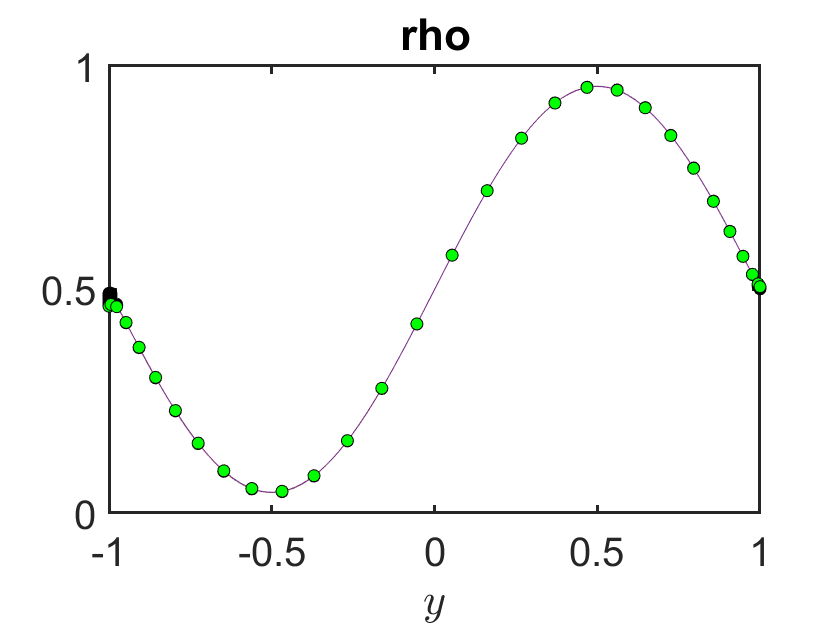
\includegraphics[width=8cm]{rho1.png}
	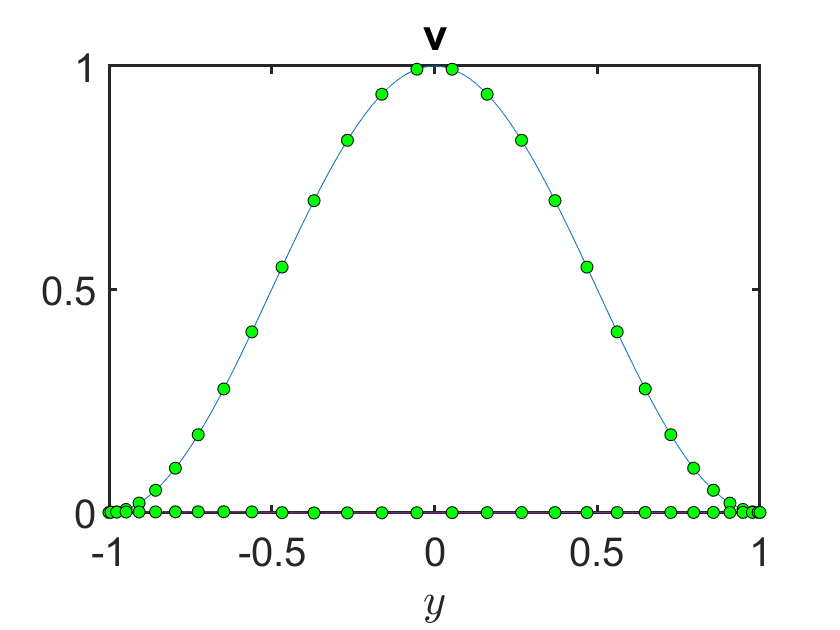
\includegraphics[width=8cm]{v1.png}
	\caption{Result for $\nabla V^{ext}_1 $ with $\gamma =5000$}
	\label{Figure1}
\end{figure}
\begin{figure}
	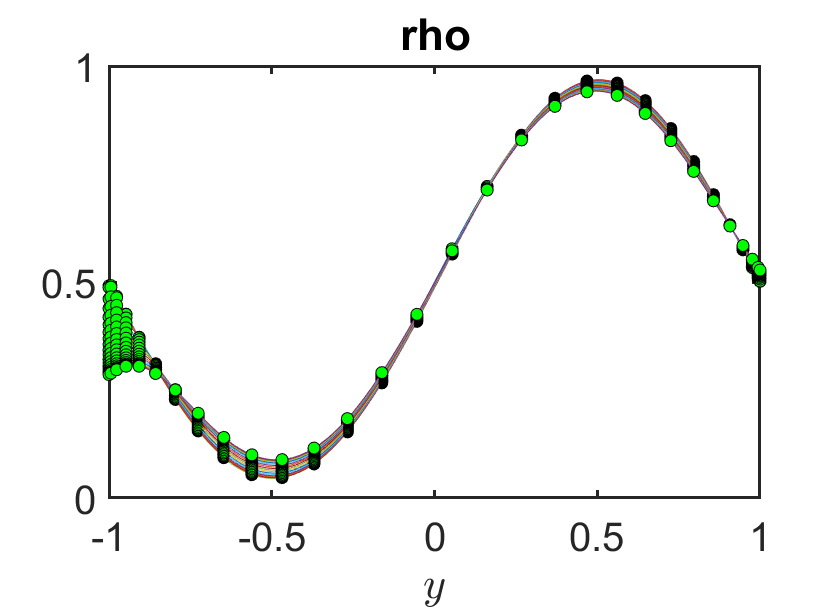
\includegraphics[width=8cm]{rho2.png}
	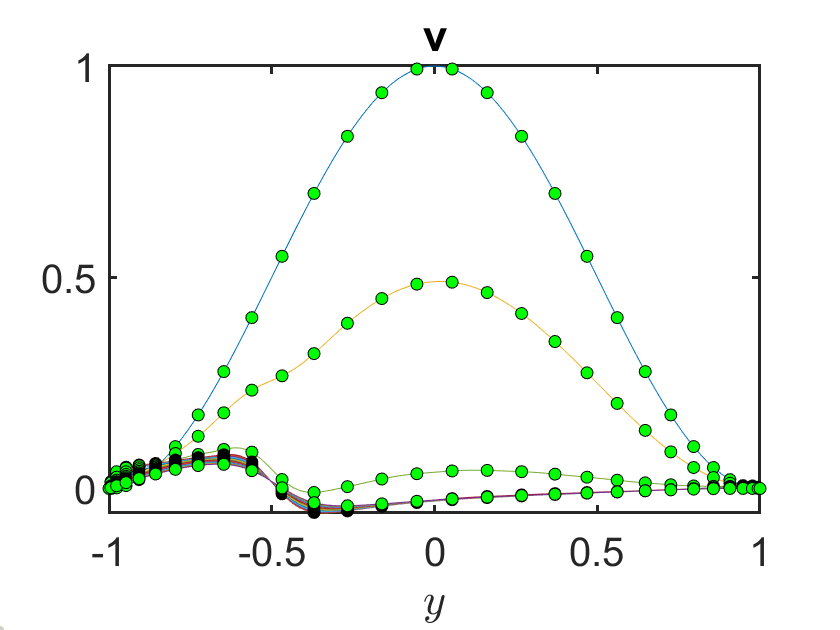
\includegraphics[width=8cm]{v2.png}
	\caption{Result for $\nabla V^{ext}_1 $ with $\gamma =100$}
	\label{Figure2}
\end{figure}
\begin{figure}
	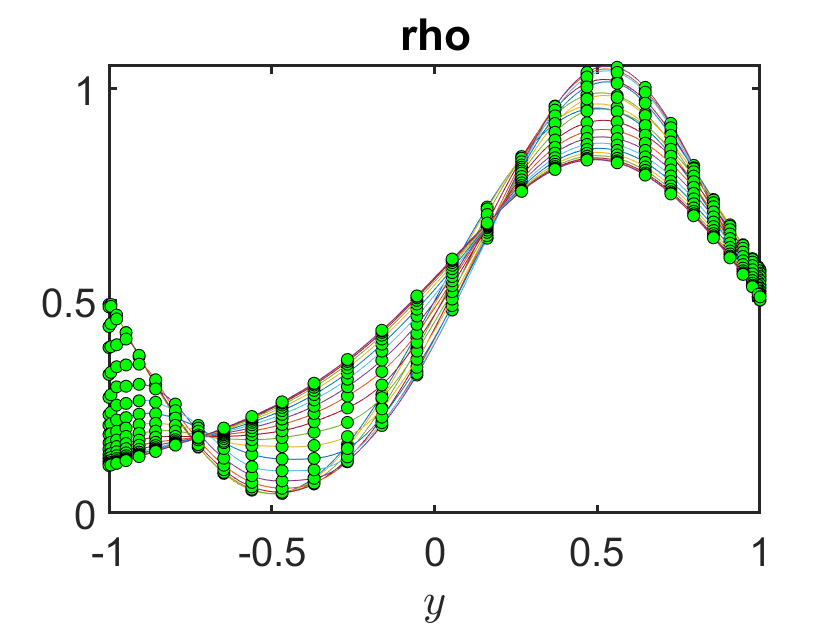
\includegraphics[width=8cm]{rho3.png}
	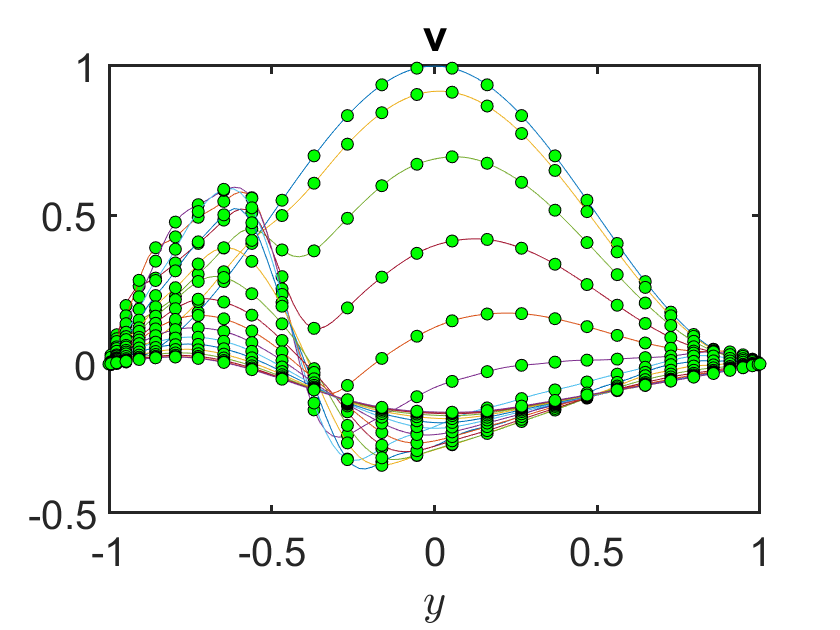
\includegraphics[width=8cm]{v3.png}
	\caption{Result for $\nabla V^{ext}_1 $ with $\gamma =10$}
	\label{Figure3}
\end{figure}

\begin{figure}
	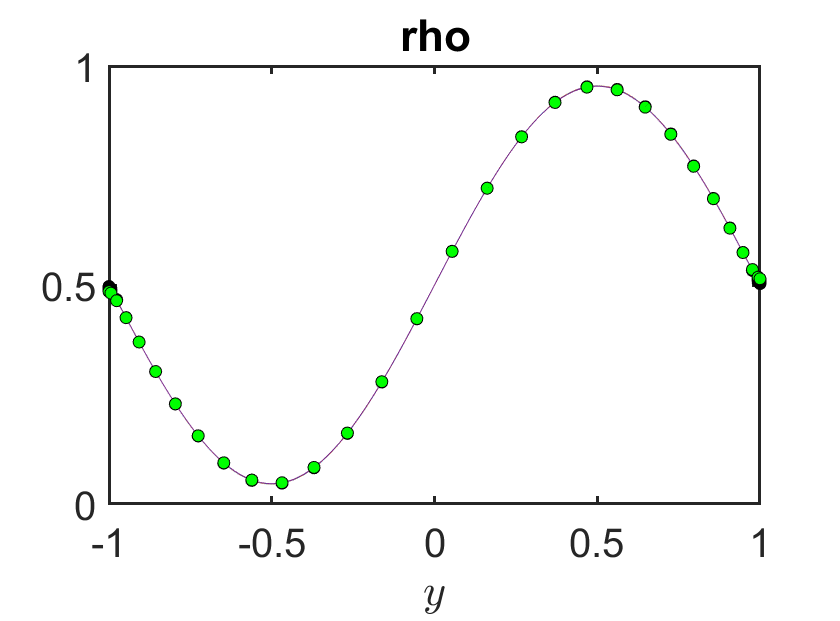
\includegraphics[width=8cm]{rho4.png}
	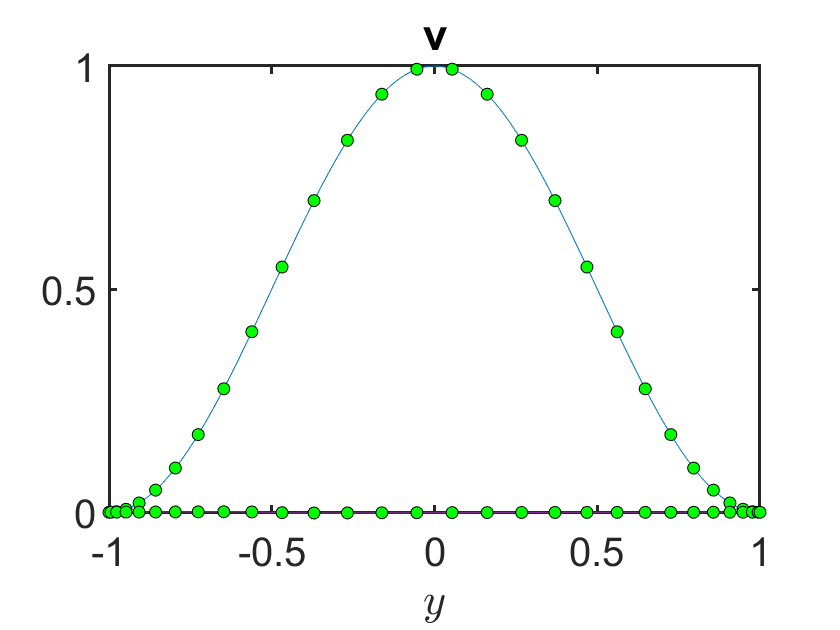
\includegraphics[width=8cm]{v4.png}
	\caption{Result for $\nabla V^{ext}_2 $ with $\gamma =5000$}
	\label{Figure4}
\end{figure}
\begin{figure}
	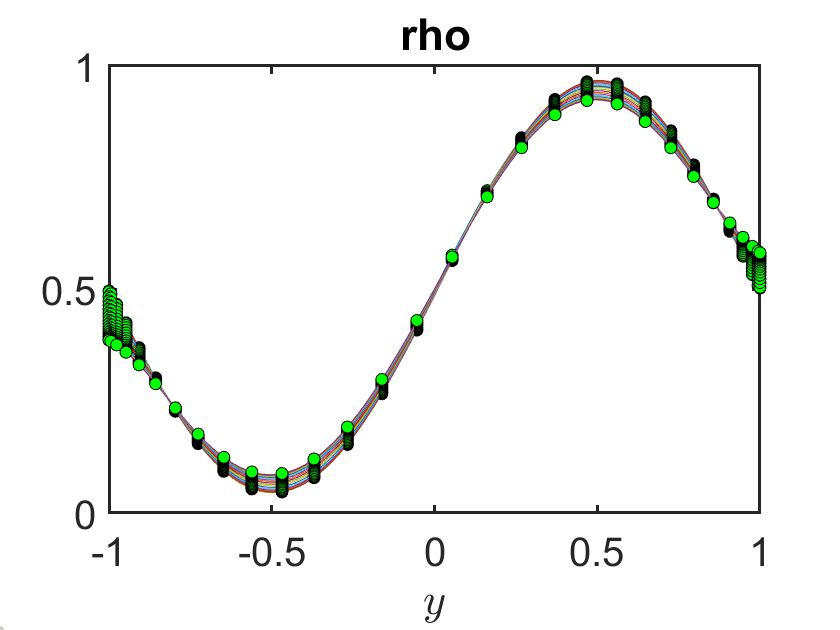
\includegraphics[width=8cm]{rho5.png}
	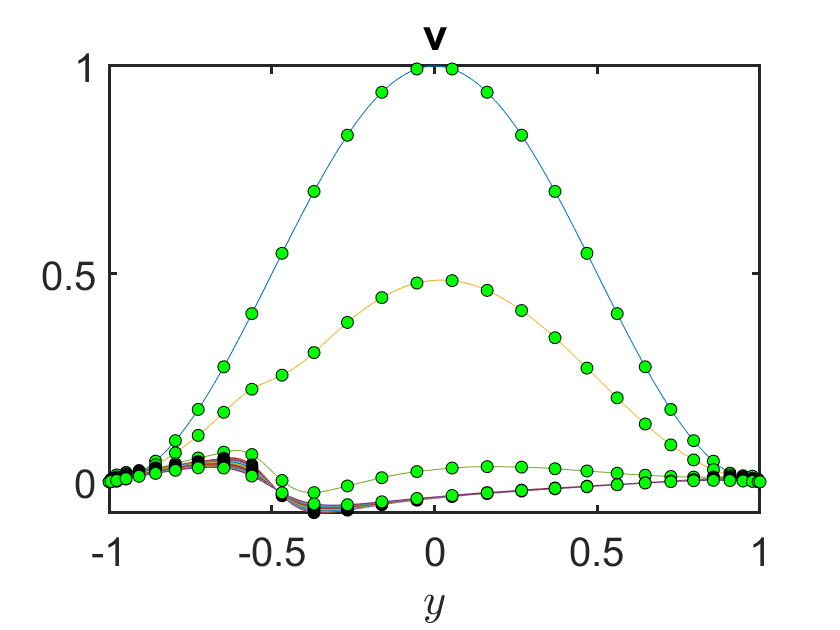
\includegraphics[width=8cm]{v5.png}
	\caption{Result for $\nabla V^{ext}_2 $ with $\gamma =100$}
	\label{Figure5}
\end{figure}
\begin{figure}
	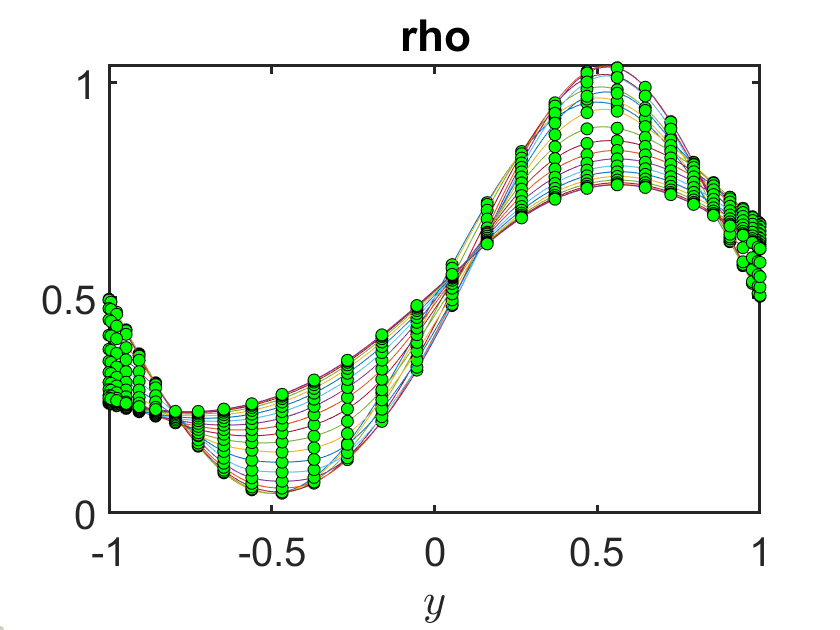
\includegraphics[width=8cm]{rho6.png}
	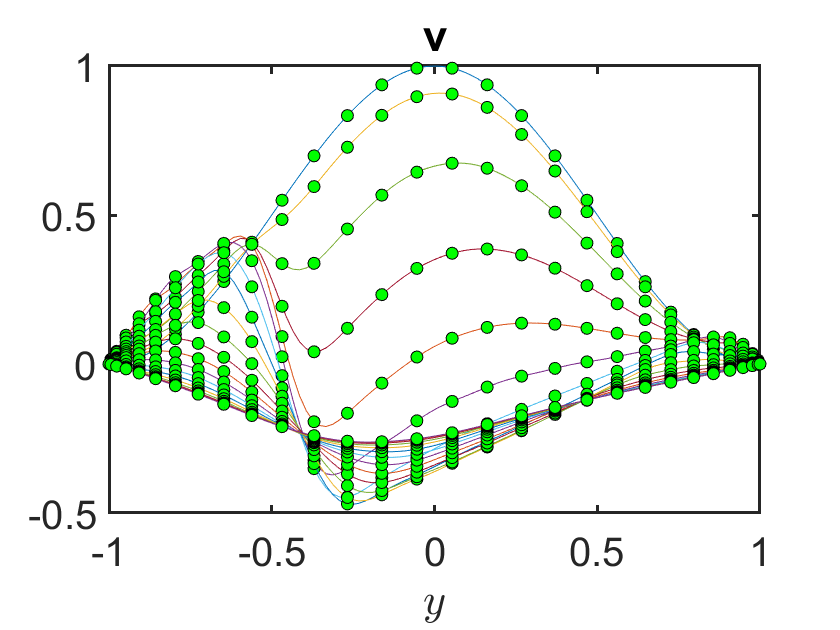
\includegraphics[width=8cm]{v6.png}
	\caption{Result for $\nabla V^{ext}_2 $ with $\gamma =10$}
	\label{Figure6}
\end{figure}

Choosing instead:
\begin{align*}
\rho_0 &= (1/1.4937)e^{-y.^2}\\
\Stav_0 &=  -y^2 + 1\\
\nabla V^{ext}_2 &= 1
\end{align*}
We get the following result for $\gamma = 10$, see Figure \ref{Figure7}.

\begin{figure}
	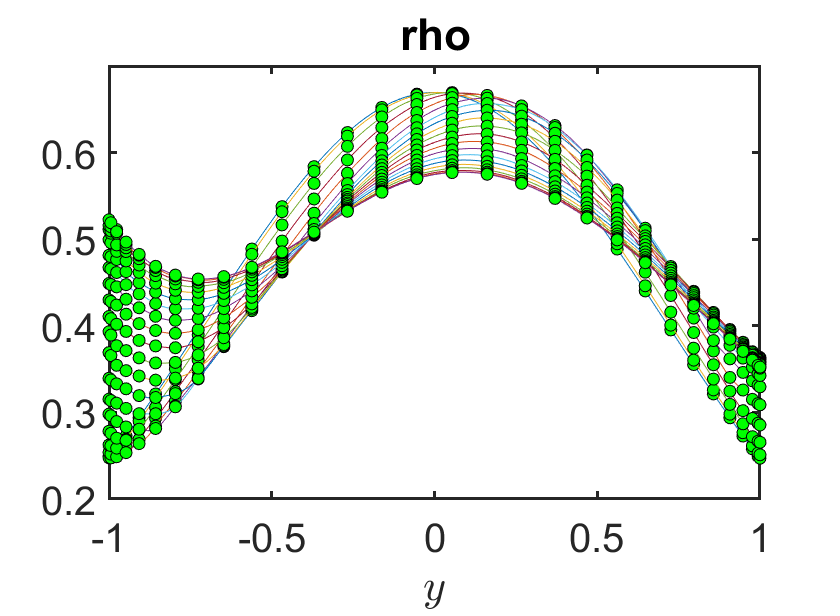
\includegraphics[width=8cm]{rho7.png}
	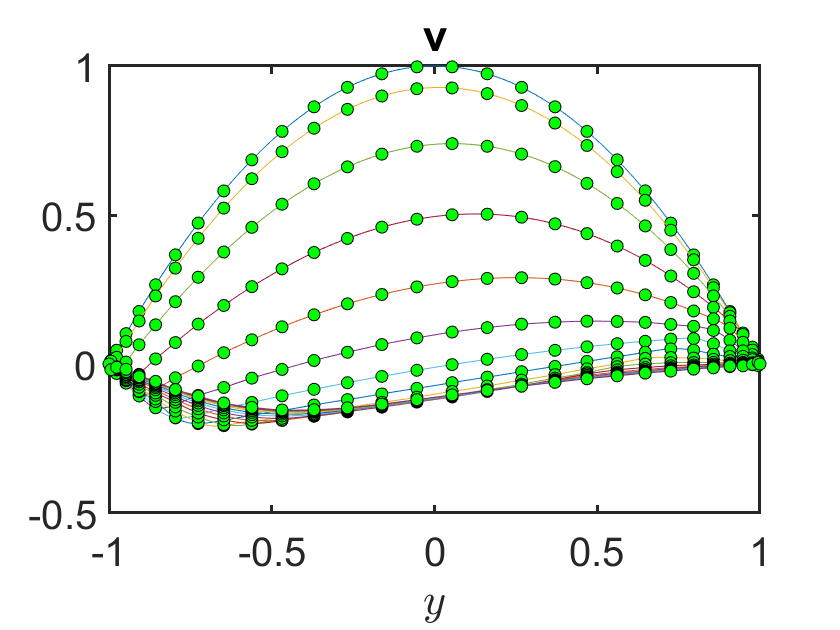
\includegraphics[width=8cm]{v7.png}
	\caption{Result for $\nabla V^{ext}_2 $ with $\gamma =10$}
	\label{Figure7}
\end{figure}



\section{Optimal Control Problem  - 'Potential Control'}
\begin{align*}
&\min_{\Sta,\Stav,\nabla V^{ext} } \quad \frac{1}{2}||\Sta - \hat \Sta||_{L_2(\Sigma)}^2 + \frac{\alpha}{2}||\Stav - \hat \Stav||_{L_2(\Sigma)}^2 +\frac{\beta}{2}||\nabla V^{ext}||_{L_2(\Sigma)}^2\\
&\text{subject to:}\\
& \frac{\partial \Stav}{\partial t} = \frac{1}{m \Sta}\bigg(- m \Sta (\Stav \cdot \nabla)\Stav - \Sta \nabla V^{ext} - \nabla \Sta - m \gamma \Sta \Stav\bigg) \ \ \ \qquad \ \ \quad\text{in} \quad \Sigma\\
&\frac{\partial \Sta}{\partial t} = - \nabla \cdot (\Sta \Stav)\\
\\
&\Sta \Stav \cdot \mathbf{n} =0	\qquad\text{on } \partial \Omega
\end{align*}

\subsection{Optimality Conditions}
Adjoint Equation 1:
\begin{align*}
& \frac{\partial \Adjb}{\partial t} = (\Sta - \hat \Sta) +m  \frac{\partial \Stav}{\partial t}\cdot \Adja + m ( (\Stav \cdot \nabla)\Stav) \cdot \Adja+ \nabla V_{ext}\cdot \Adja -\nabla\cdot \Adja  - \ \nabla \Adjb \cdot \Stav  \\
&+ m \gamma \Stav \cdot \Adja  \qquad\qquad\qquad\qquad\qquad \text{in} \quad \Sigma \\
& \Adja \cdot \mathbf{n} = 0 \qquad \text{on} \quad \partial \Sigma\\
&\Adjb(T) = {0}
\end{align*}
Adjoint Equation 2:
\begin{align*}
&   \frac{\partial \Adja}{\partial t}  = \frac{1}{m \Sta} \bigg(\alpha(\Stav - \hat \Stav)   - m \frac{\partial \Sta}{\partial t} \Adja 
-\Sta\nabla \Adjb +m \Sta (\nabla \Stav)^\top \Adja +m \gamma \Sta \Adja \\
&-m \Sta (\Stav \cdot \nabla)\Adja - m \Sta (\nabla \cdot \Stav)\Adja  - m (\Stav \cdot \nabla \Sta)\Adja \bigg)\ \qquad\qquad \qquad\text{in} \quad \Sigma\\
&\Adja(T)=\mathbf{0}.
\end{align*}
Gradient Equation:
\begin{align*}
\nabla V^{ext} = \frac{1}{\beta} \rho \mathbf{p}
\end{align*}
\subsection{First Results (provided correct implementation?)}
Choosing ($\rho$ mass $1$, $\Stav$ BCs zero, $\nabla V^{ext}$ sort of in line with gradient eqation, i.e. something containing $\rho$ and final time condition for $\mathbf{p}$ satisfied):
\begin{align*}
\rho_0 &= (1/2.2)(\sin(\pi y) + 1.1)\\
\Stav_0 &=  -y^2 + 1\\
\nabla V^{ext}_3 &= (1/\beta)(e^{T}-e^t)((1/2)\cos(\pi y) +1/2)
\end{align*}
The targets are:
\begin{align*}
&rhoTarget = (1-t)(1/2.2)(\sin(\pi y) + 1.1) +  t(1/1.4937)\exp(-y^2)\\
&vTarget = (1 - t)(-y^2 + 1) + t(((1/2)\cos(\pi y) + 1/2))
\end{align*}
Then choosing very easy settings: $\beta = 10$, ODE tols $= 10^{-6}$, optimality tols $= 10^{-3}$, $\gamma = 5$ and $\alpha =m=1$, $N=30$, $n=20$, $\lambda = 0.01$ this converges, see Figure \ref{Figure8}. Converges in around $700 - 800$ iterations but the results are $J_{FW} = 0.6868$, $J_{Opt} = 2.1045$. So something is wrong. (And smaller $\beta$ diverge quickly.)

\begin{figure}
	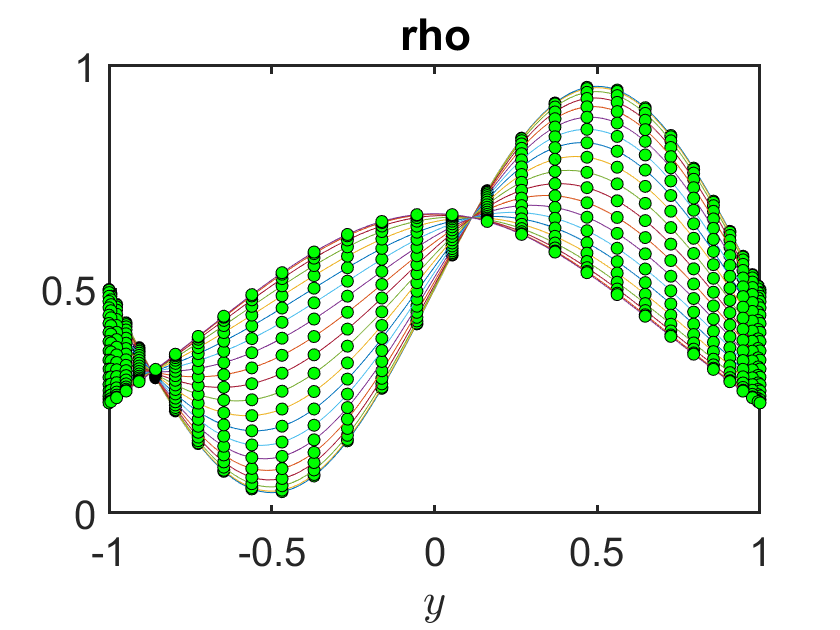
\includegraphics[width=7cm]{rhoHat1.png}
	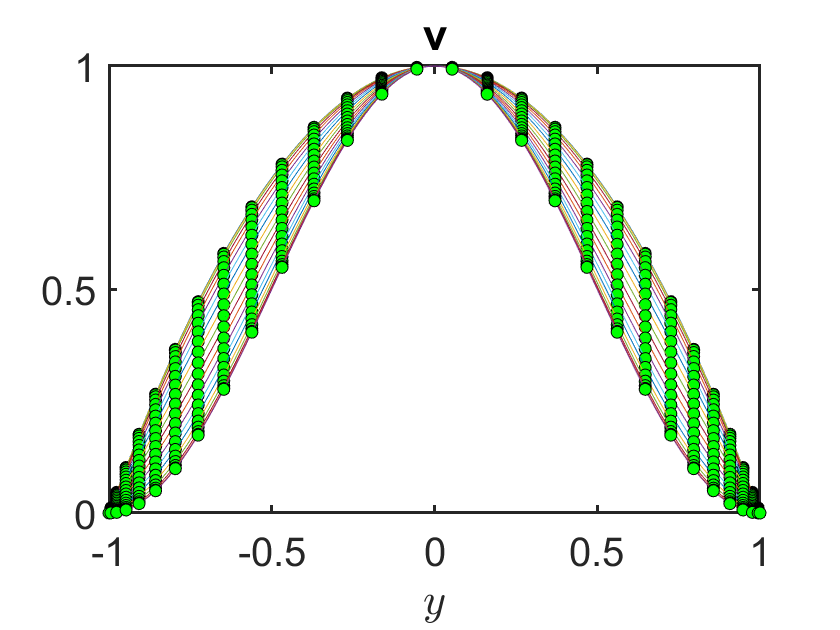
\includegraphics[width=7cm]{vHat1.png}\\
	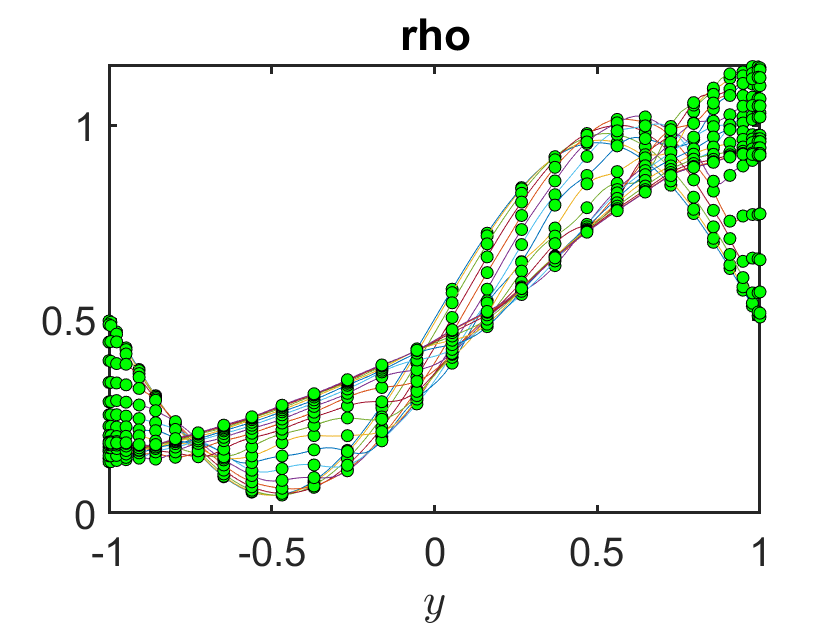
\includegraphics[width=5cm]{FWrho1.png}
	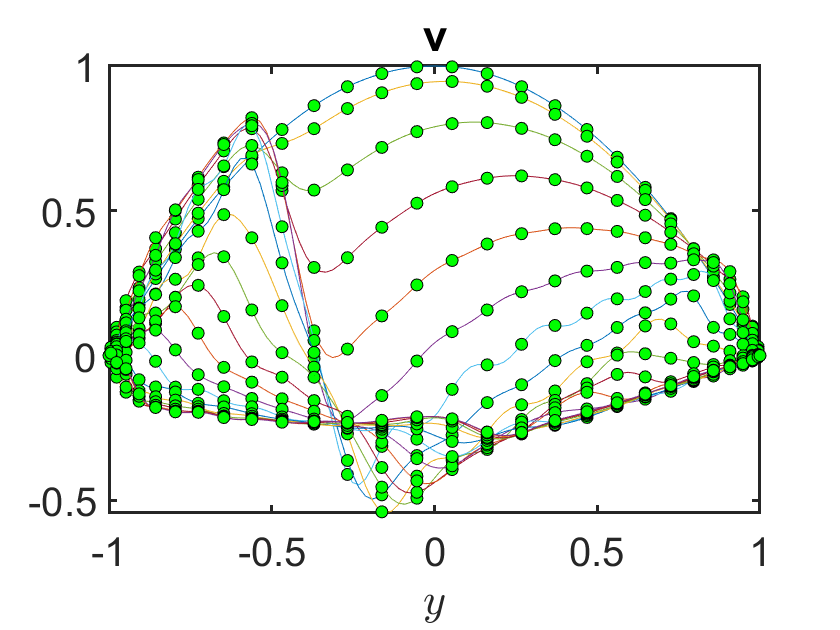
\includegraphics[width=5cm]{FWv1.png}
	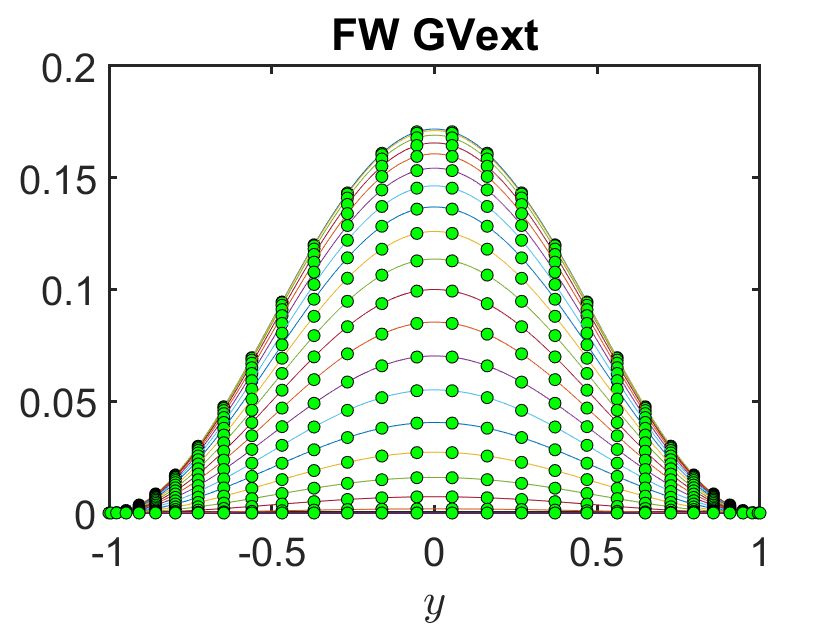
\includegraphics[width=5cm]{FWCont1.png}\\
	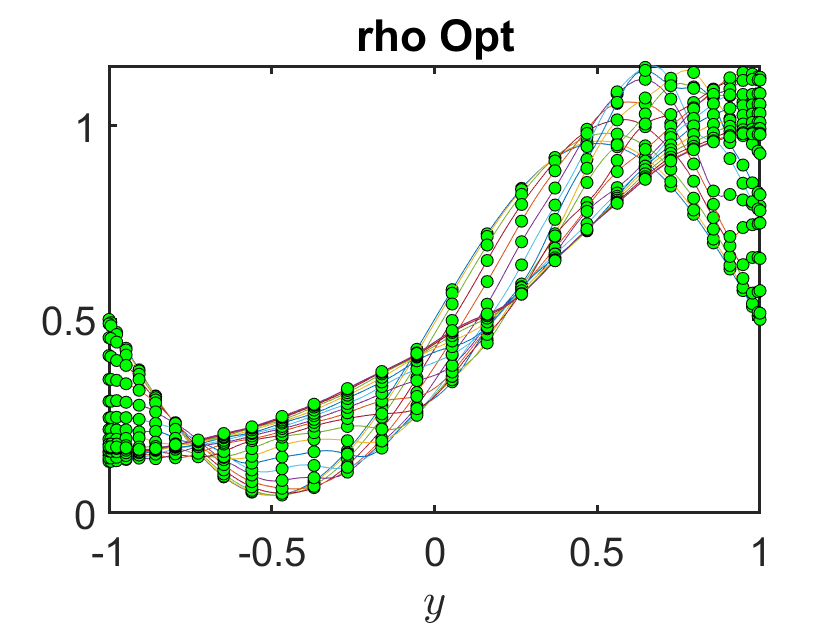
\includegraphics[width=5cm]{Optrho1.png}
	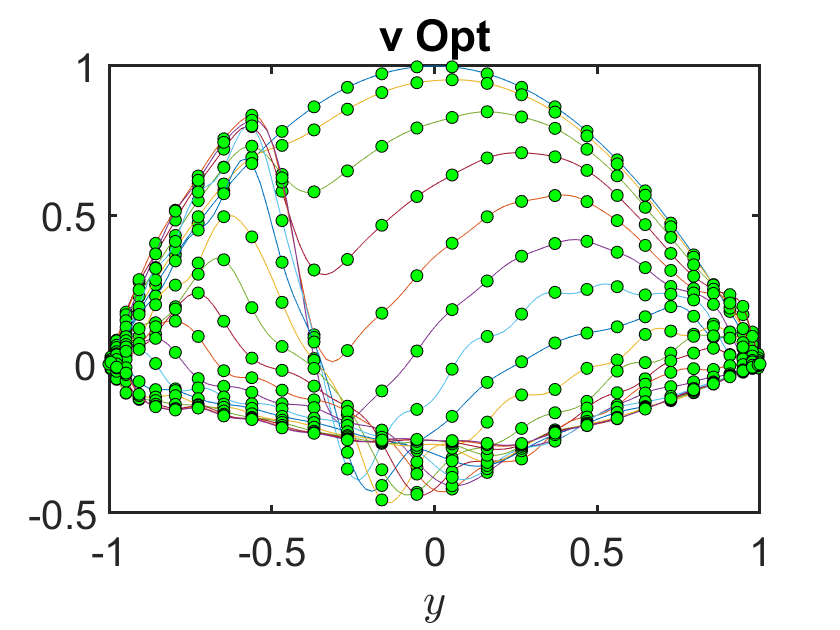
\includegraphics[width=5cm]{Optv1.png}
	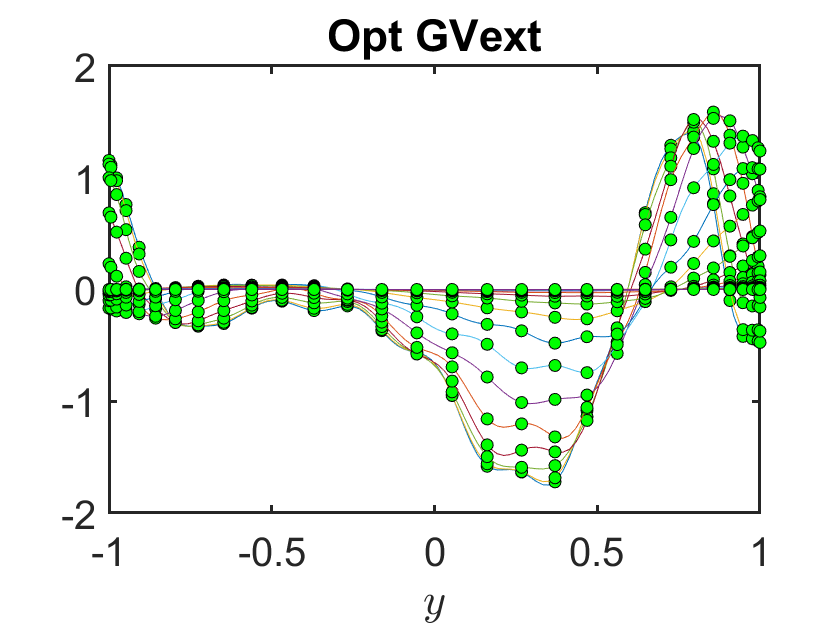
\includegraphics[width=5cm]{OptCont1.png}
	\caption{targets (top), FW Result OCP (middle), Opt (bottom) for $\nabla V^{ext}_3 $ with $\gamma =10$}
	\label{Figure8}
\end{figure}

Next try rhoHat, vHat from forward problem. The results are $J_{FW} = 0.0466$ and $J_{Opt} = 6.5415e-04$, so that's good. the results are in Figure \ref{Figure9}. It converges in about $500$ iterations.

\begin{figure}
	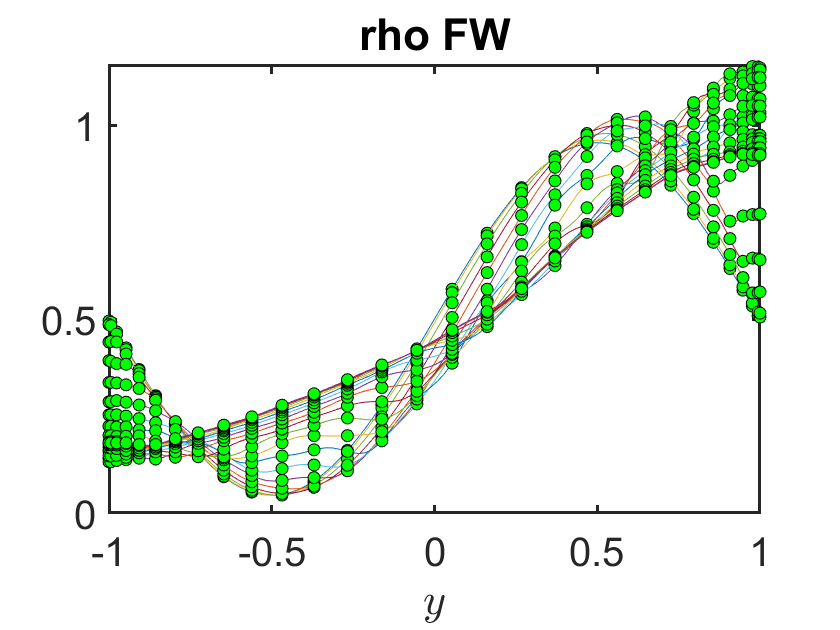
\includegraphics[width=5cm]{FWrho3.png}
	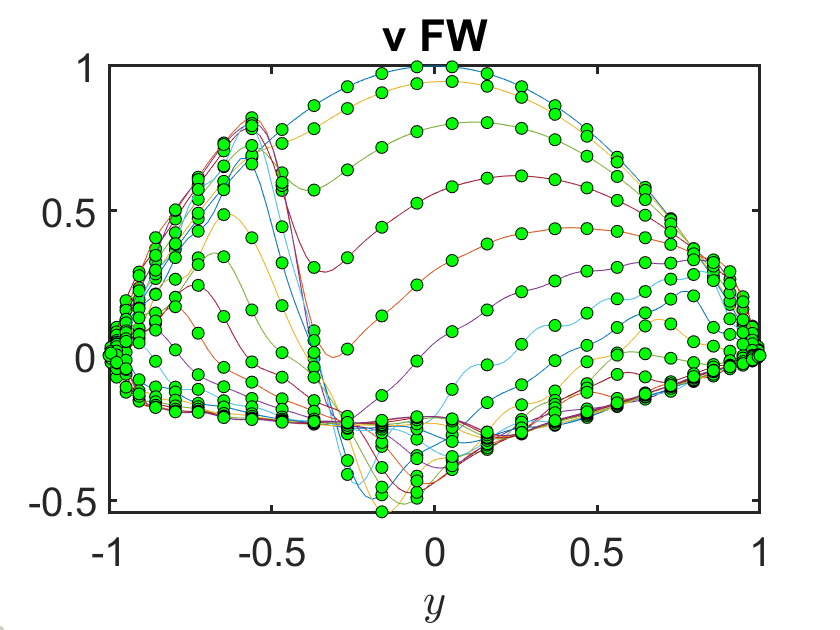
\includegraphics[width=5cm]{FWv3.png}
	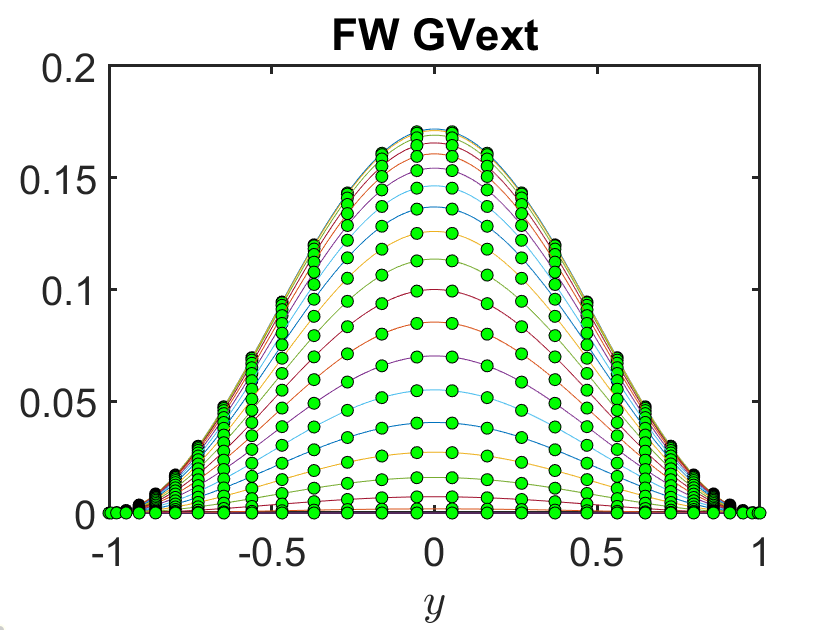
\includegraphics[width=5cm]{FWCont3.png}\\
	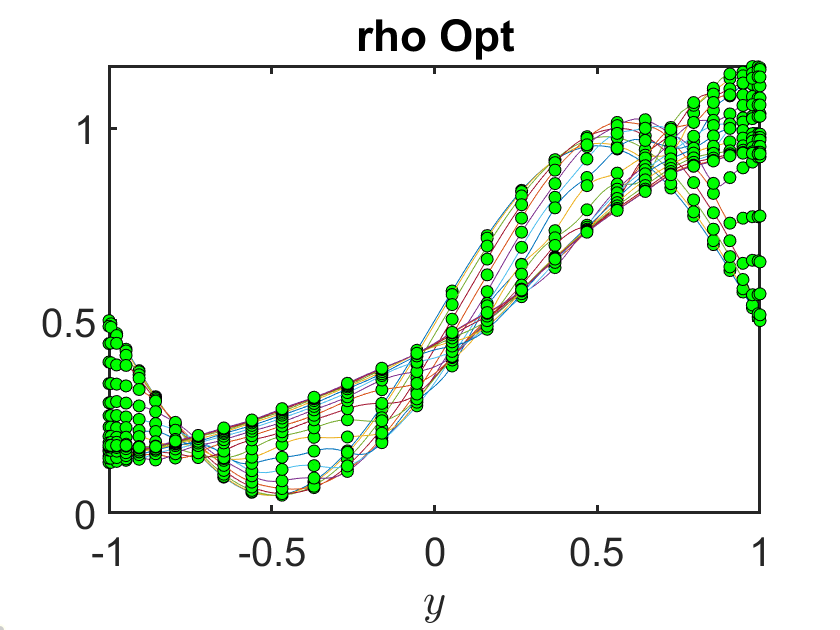
\includegraphics[width=5cm]{Optrho3.png}
	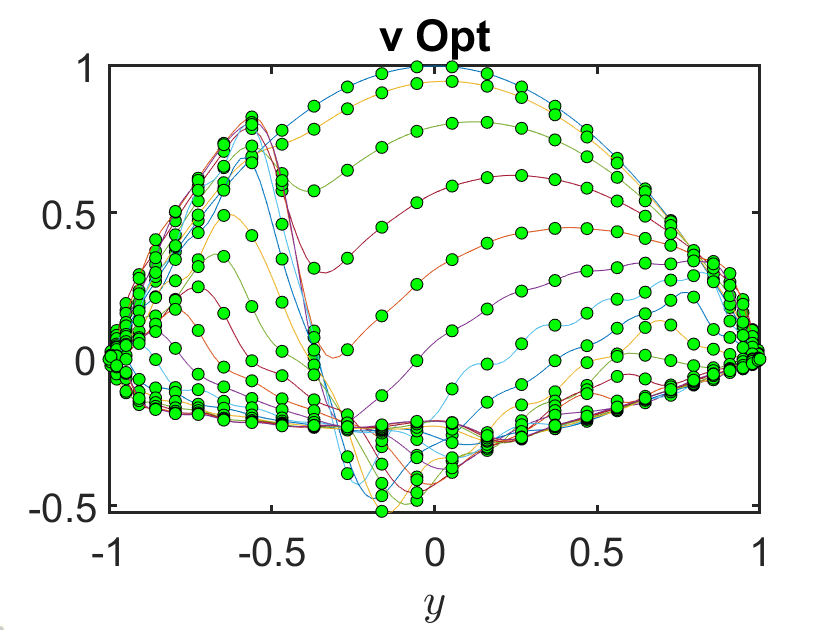
\includegraphics[width=5cm]{Optv3.png}
	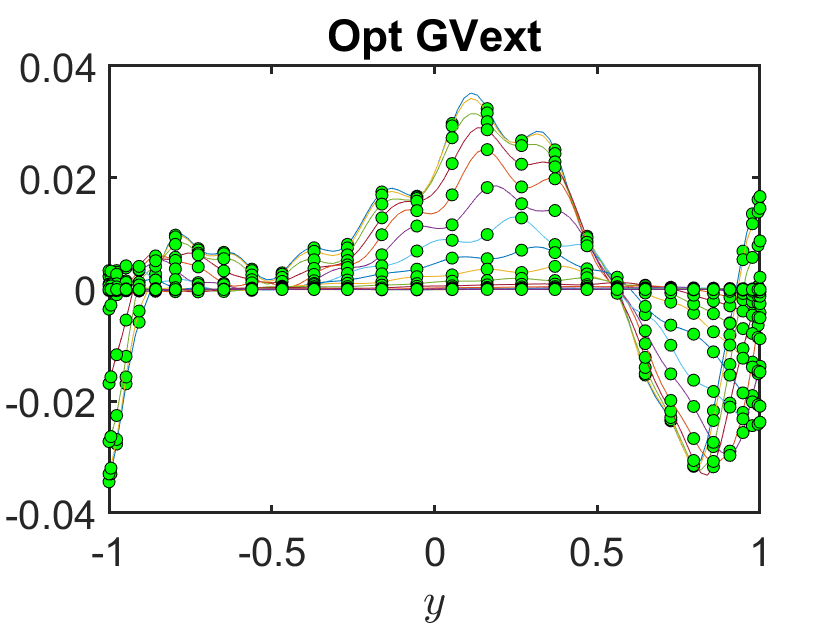
\includegraphics[width=5cm]{OptCont3.png}
	\caption{FW Result OCP (top), Opt (bottom) for $\nabla V^{ext}_3 $ with $\beta =10$ and FW result is target}
	\label{Figure9}
\end{figure}
For $\beta = 1$ this converges too, but it takes $1000$ iterations and looks much more unstable, see Figure \ref{Figure10}.
\begin{figure}
	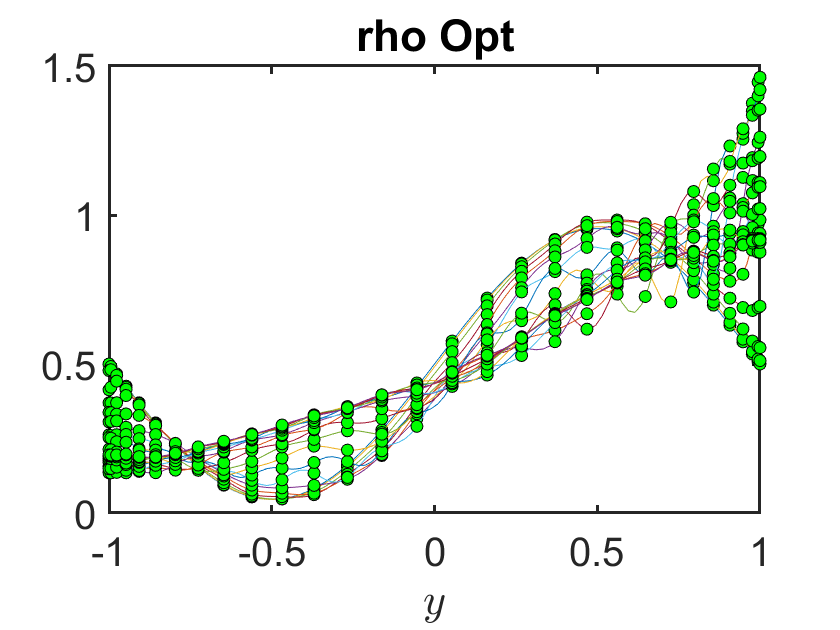
\includegraphics[width=5cm]{Optrho4.png}
	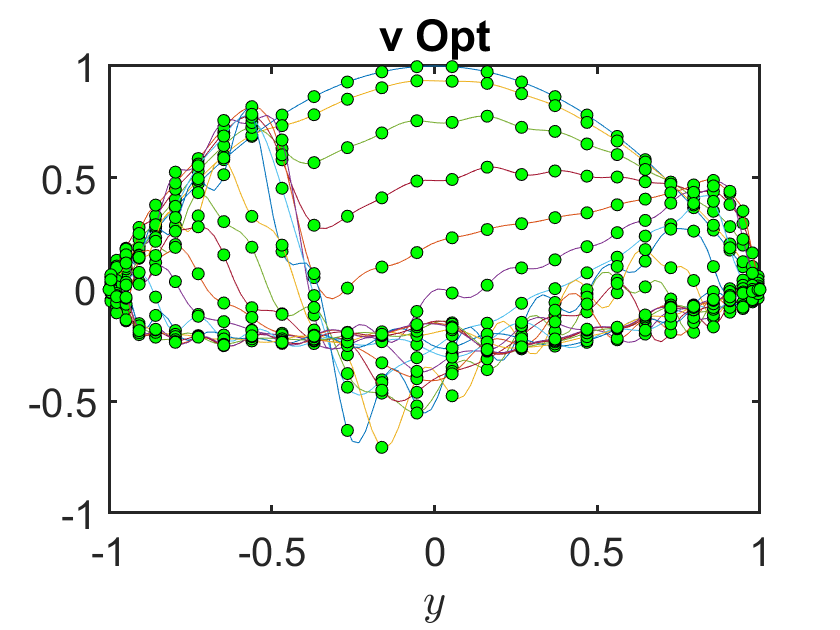
\includegraphics[width=5cm]{Optv4.png}
	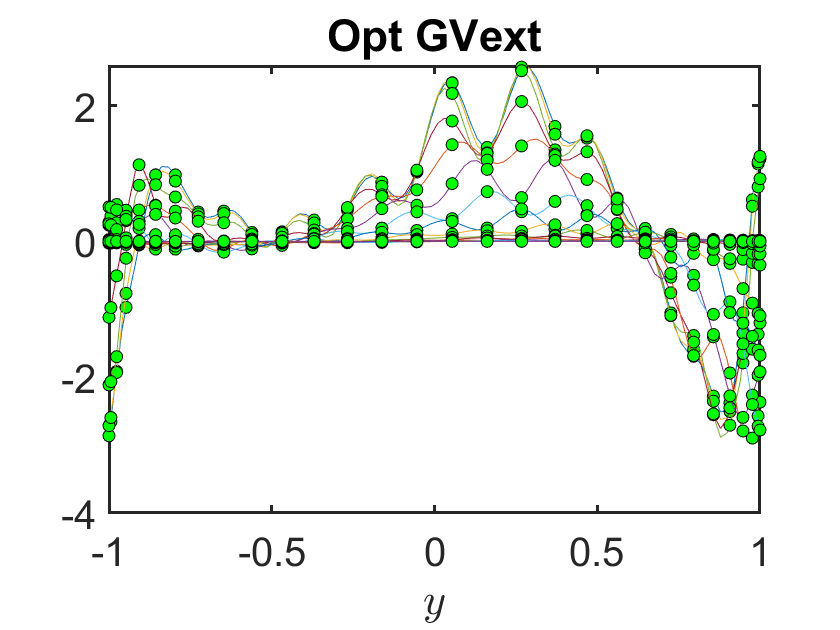
\includegraphics[width=5cm]{OptCont4.png}
	\caption{FW Result OCP (top), Opt (bottom) for $\nabla V^{ext}_3 $ with $\beta =1$ and FW result is target}
	\label{Figure10}
\end{figure}
With these configurations $\beta = 10^{-1}$ doesn't even work for the forward problem. It is clear that the choice of initial inputs isn't very good, some of the solutions aren't so stable. However, it doesn't help to increase the points or decrease the tolerances.
\subsection{Change $\nabla V^{ext}$}
Change it to be independent of $\beta$ this stabilizes the forward problem.
Consequently also the OCP.
Choose same as before, minus beta dependence.
\begin{align*}
\rho_0 &= (1/2.2)(\sin(\pi y) + 1.1)\\
\Stav_0 &=  -y^2 + 1\\
\nabla V^{ext}_3 &= (e^{T}-e^t)((1/2)\cos(\pi y) +1/2)
\end{align*}
The targets come from forward problem.
$\beta = 10^{-1}$ still doesn't work (diverges). Observation (again): the forward problem likes larger $\gamma$, but the OCP diverges faster if $\gamma$ is larger. Still works for $\beta = 1$.
\section{Optimal Control Problem - Force Control}
The OCP:
\begin{align*}
&\min_{\Sta,\Stav,\Con } \quad \frac{1}{2}||\Sta - \hat \Sta||_{L_2(\Sigma)}^2 + \frac{\alpha}{2}||\Stav - \hat \Stav||_{L_2(\Sigma)}^2 +\frac{\beta}{2}||\Con||_{L_2(\Sigma)}^2\\
&\text{subject to:}\\
& \frac{\partial \Stav}{\partial t} = \frac{1}{m \Sta}\bigg(- m \Sta (\Stav \cdot \nabla)\Stav - \Sta \nabla V_{ext} - \nabla \Sta - m \gamma \Sta \Stav - \Con\bigg) \ \ \ \qquad \ \ \quad\text{in} \quad \Sigma\\
&\frac{\partial \Sta}{\partial t} = - \nabla \cdot (\Sta \Stav)\\
\\
&\Sta \Stav \cdot \mathbf{n} =0	\qquad\text{on } \partial \Omega
\end{align*}

\subsection{Optimality Conditions}
Adjoint Equation 1:
\begin{align*}
& \frac{\partial \Adjb}{\partial t} = (\Sta - \hat \Sta) +m  \frac{\partial \Stav}{\partial t}\cdot \Adja + m ( (\Stav \cdot \nabla)\Stav) \cdot \Adja+ \nabla V_{ext}\cdot \Adja -\nabla\cdot \Adja  - \ \nabla \Adjb \cdot \Stav  \\
&+ m \gamma \Stav \cdot \Adja  \qquad\qquad\qquad\qquad\qquad \text{in} \quad \Sigma \\
& \Adja \cdot \mathbf{n} = 0 \qquad \text{on} \quad \partial \Sigma\\
&\Adjb(T) = {0}
\end{align*}
Adjoint Equation 2:
\begin{align*}
&   \frac{\partial \Adja}{\partial t}  = \frac{1}{m \Sta} \bigg(\alpha(\Stav - \hat \Stav)   - m \frac{\partial \Sta}{\partial t} \Adja 
-\Sta\nabla \Adjb +m \Sta (\nabla \Stav)^\top \Adja +m \gamma \Sta \Adja \\
&-m \Sta (\Stav \cdot \nabla)\Adja - m \Sta (\nabla \cdot \Stav)\Adja  - m (\Stav \cdot \nabla \Sta)\Adja \bigg)\ \qquad\qquad \qquad\text{in} \quad \Sigma\\
&\Adja(T)=\mathbf{0}.
\end{align*}
Gradient Equation:
\begin{align*}
\Con = - \frac{1}{\beta}\mathbf{p}
\end{align*}


\subsection{First Results (with care)}
Choose:
\begin{align*}
&\rho_0 = 5(1/2.2)(\sin(\pi y) + 1.1)\\
&\Stav_0 = -y^2 + 1\\
&\Con = (T-t)y\\
&\nabla V^{ext} = \cos(\pi y)
\end{align*}
Note that the control is $\Con$ and $\nabla V^{ext}$ is just an input now.
The friction coefficient is set to $10$ now because a lower value results in failing the forward problem. Higher values mess with the convergence of the optimality system. We have $\beta = 10$ and $\lambda = 0.01$. Choose again $10^{-6}/10^{-3}$ tolerances.
This converges in around $800$ iterations. The result is $J_{FW} = 1.1111$ and $J_{Opt} = 0.6193$. Figure \ref{Figure11} shows the result. The targets are the forward results. It can be seen that the optimal control is becoming 'wiggly' at times.

\begin{figure}
	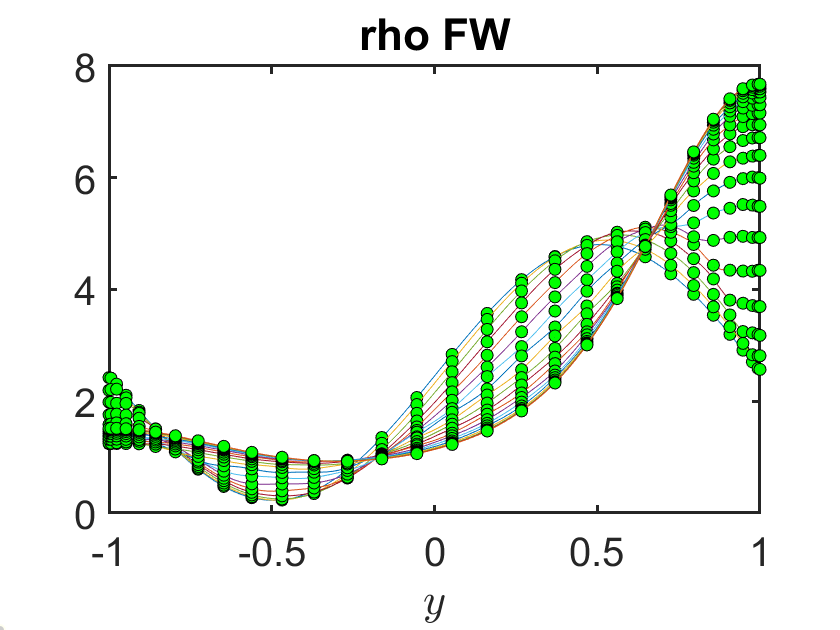
\includegraphics[width=5cm]{FWrho4.png}
	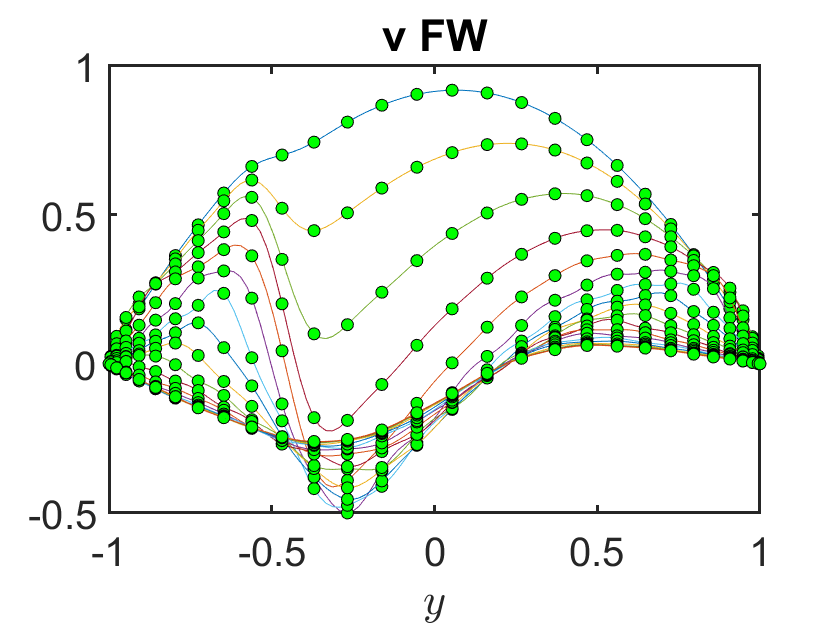
\includegraphics[width=5cm]{FWv4.png}
	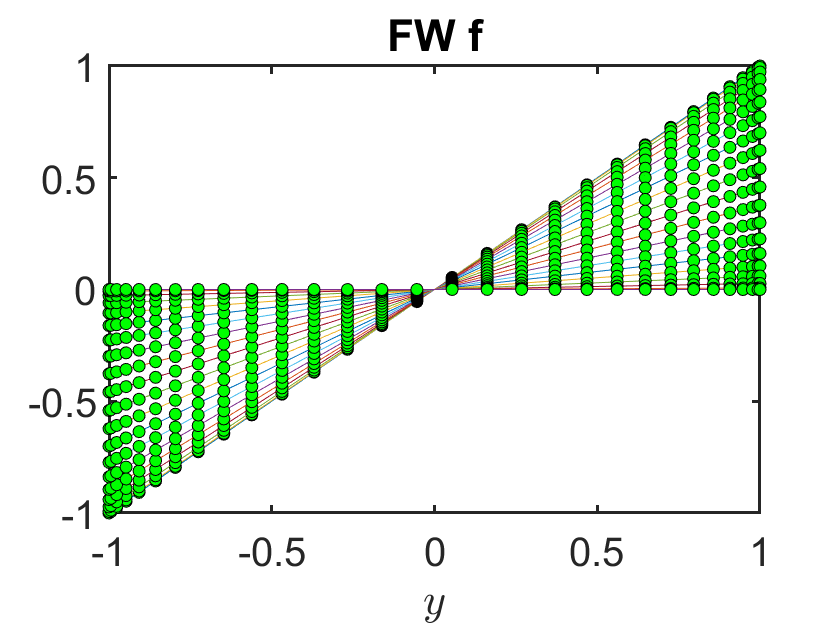
\includegraphics[width=5cm]{FWCont4.png}\\
	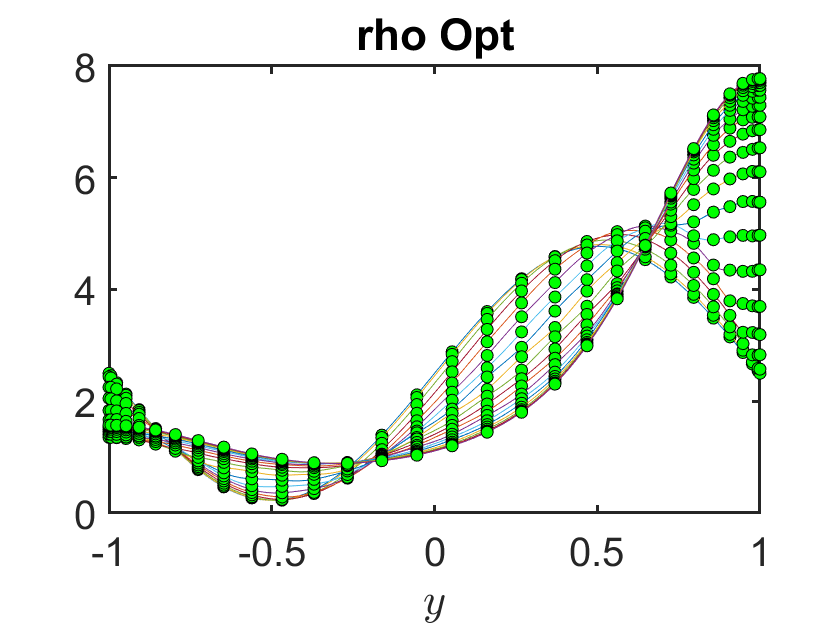
\includegraphics[width=5cm]{Optrho5.png}
	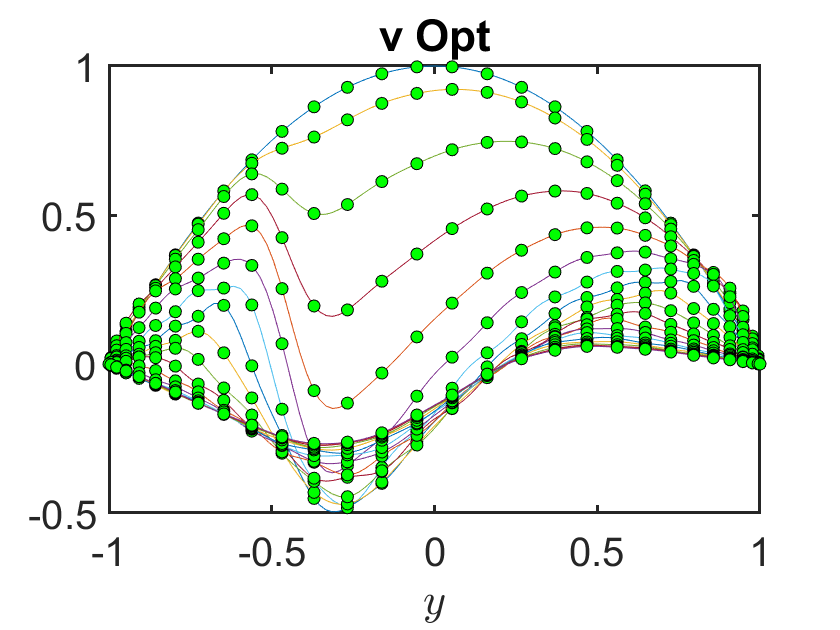
\includegraphics[width=5cm]{Optv5.png}
	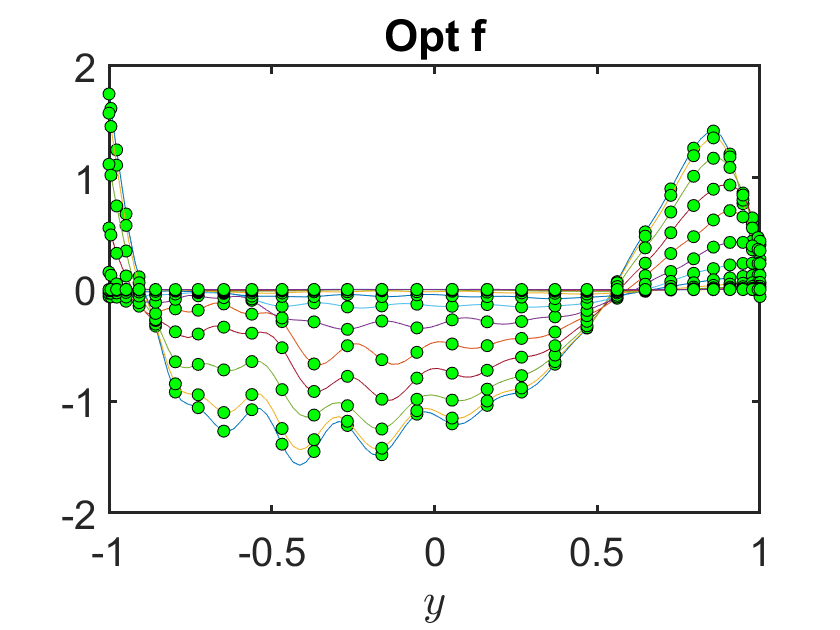
\includegraphics[width=5cm]{OptCont5.png}
	\caption{FW Result OCP (top), Opt (bottom) for $\Con $, force control, with $\gamma =10$ and FW result is target}
	\label{Figure11}
\end{figure}
Redoing this exact problem with $N=60$ and $n=50$, it takes almost $1000$ iterations to converge, but looks a little more stable, see Figure \ref{Figure12}.
The result is $J_{FW} = 1.1111$ and $J_{Opt} = 0.8655$. This is considerably different from the case with less points. So it has to be checked how many points are necessary. We can see that one of the suspected problems is that the control becomes very steep on the boundaries.
\begin{figure}
	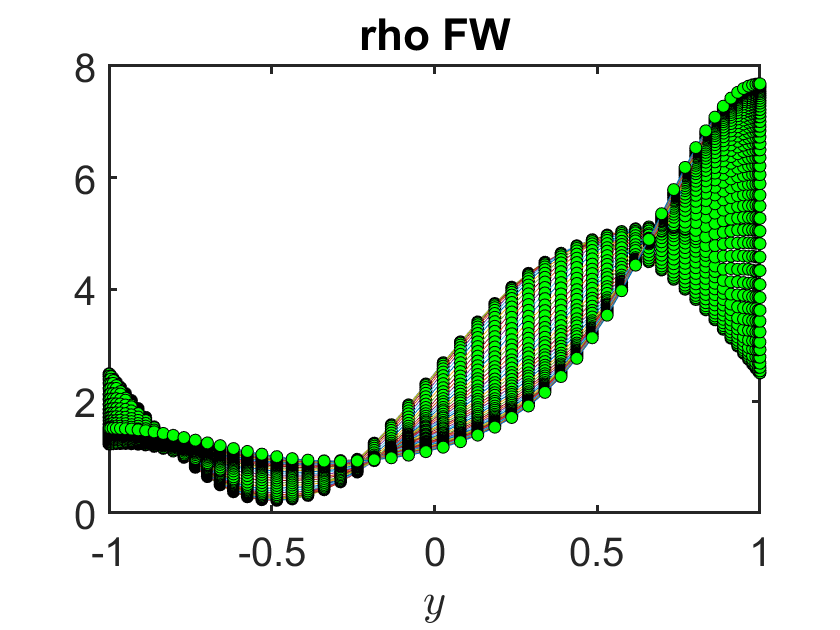
\includegraphics[width=5cm]{FWrho6.png}
	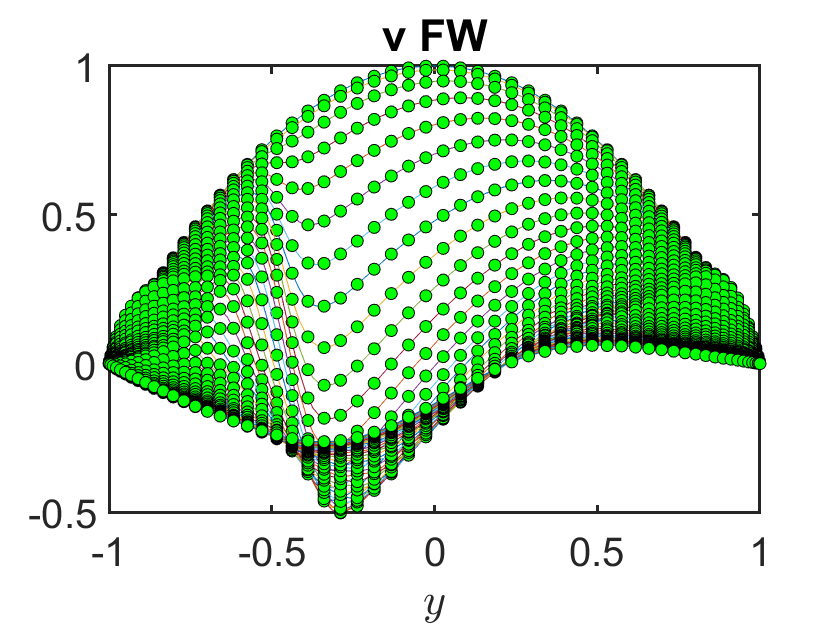
\includegraphics[width=5cm]{FWv6.png}
	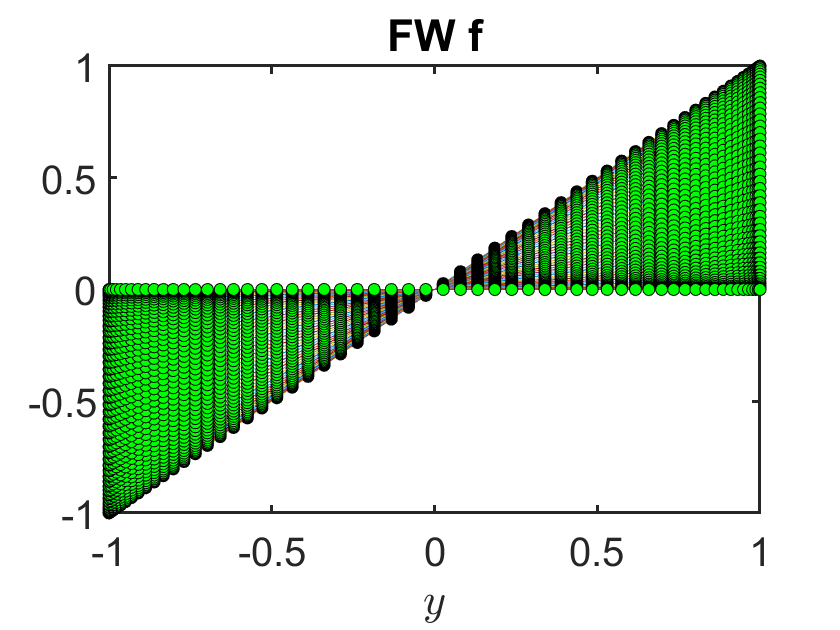
\includegraphics[width=5cm]{FWCont6.png}\\
	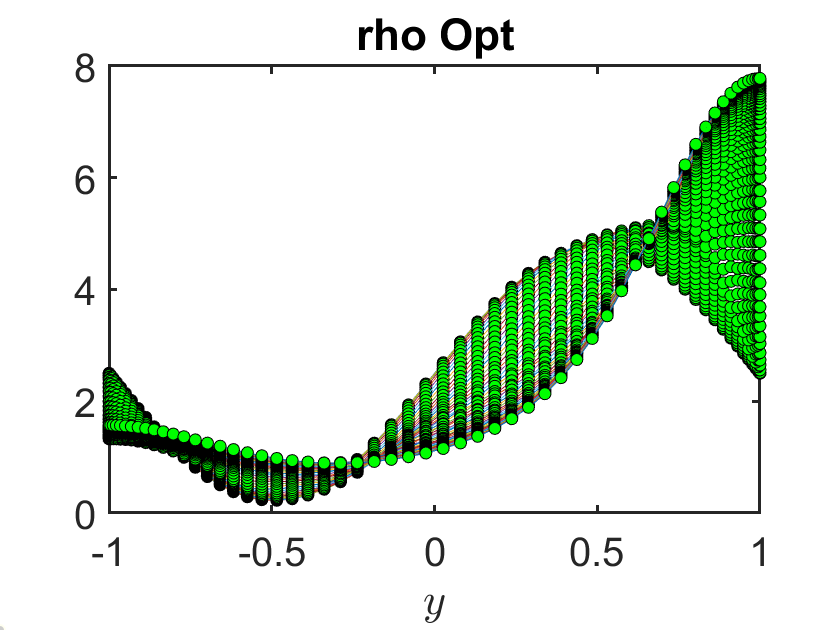
\includegraphics[width=5cm]{Optrho6.png}
	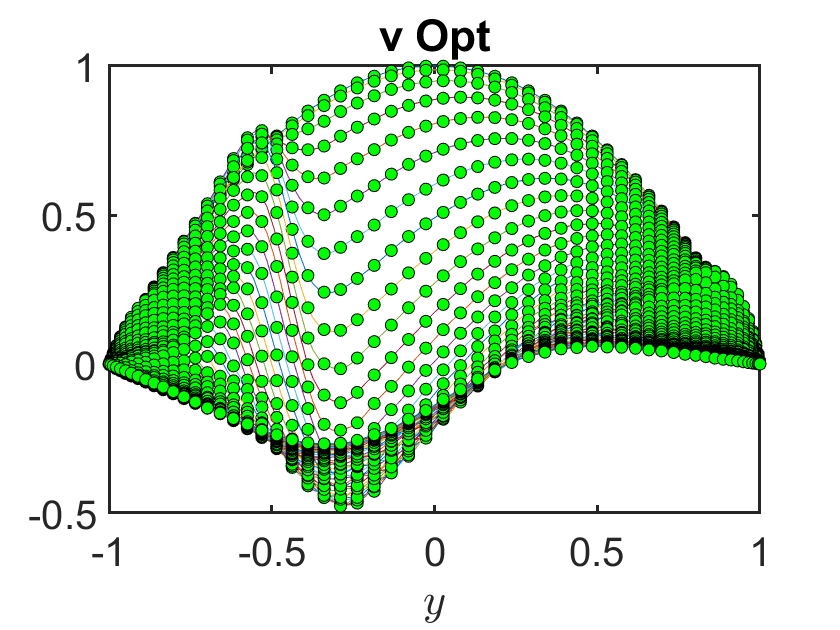
\includegraphics[width=5cm]{Optv6.png}
	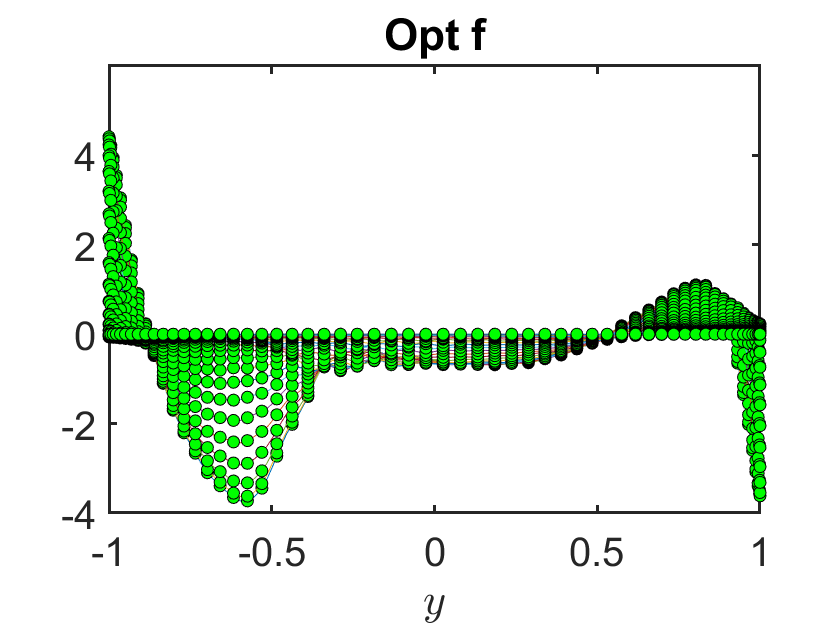
\includegraphics[width=5cm]{OptCont6.png}
	\caption{FW Result OCP (top), Opt (bottom) for $\Con $, force control, with $\gamma =10$ and FW result is target, more points}
	\label{Figure12}
\end{figure}

\subsection{Quick sanity check}
After solving the above, we get $\Con_{Opt}$. Now, giving the code this optimal value of $\Con$, with the same target, ICs etc, we expect so solve the problem in one iteration. This indeed happens. So at least we found something that the system considers optimal, what ever that may mean in practice.

\end{document}